\documentclass[a4paper,14pt]{extarticle} 
\usepackage[a4paper,top=1.5cm, bottom=1.5cm, left=2cm, right=1cm]{geometry}
%\usepackage[T2A]{fontenc}
%\usepackage[english, russian]{babel}
\usepackage{graphicx}
\DeclareGraphicsExtensions{.pdf,.png,.jpg}

\usepackage{fontspec}
\setmainfont{Times New Roman}
\setsansfont{FreeSans}
\setmonofont{FreeMono}
\renewcommand{\baselinestretch}{1.5}
\usepackage{polyglossia}
\setdefaultlanguage{russian}
\setotherlanguages{english,russian}
\usepackage{setspace}
\usepackage[many]{tcolorbox}
\usepackage{listings}
\usepackage{xcolor}

\definecolor{codegreen}{rgb}{0,0.6,0}
\definecolor{codegray}{rgb}{0.5,0.5,0.5}
\definecolor{codepurple}{rgb}{0.58,0,0.82}
\definecolor{backcolour}{rgb}{0.95,0.95,0.92}

\lstdefinestyle{mystyle}{
    backgroundcolor=\color{backcolour},   
    keywordstyle=\color{magenta},
    numberstyle=\tiny\color{codegray},
    stringstyle=\color{codepurple},
    basicstyle=\ttfamily\footnotesize,
    breakatwhitespace=false,         
    breaklines=true,                 
    captionpos=b,                    
    keepspaces=true,                 
    numbers=left,                    
    numbersep=5pt,                  
    showspaces=false,                
    showstringspaces=false,
    showtabs=false,                  
    tabsize=2
}

\lstset{style=mystyle}

\begin{document}
    \begin{center}
        \thispagestyle{empty}
        \begin{singlespace}
        ФЕДЕРАЛЬНОЕ АГЕНТСТВО СВЯЗИ

        ФЕДЕРАЛЬНОЕ ГОСУДАРСТВЕННОЕ БЮДЖЕТНОЕ ОБРАЗОВАТЕЛЬНОЕ

        УЧРЕЖДЕНИЕ ВЫСШЕГО ОБРАЗОВАНИЯ

        «САНКТ-ПЕТЕРБУРГСКИЙ ГОСУДАРСТВЕННЫЙ УНИВЕРСИТЕТ ТЕЛЕКОММУНИКАЦИЙ ИМ. ПРОФ. М.А. БОНЧ-БРУЕВИЧА»

        (СПбГУТ)
        \end{singlespace}
        \vspace{-1ex}
        \rule{\textwidth}{0.4pt}
        \vspace{-5ex}

        Факультет \underline{Инфокоммуникационных сетей и систем}

        Кафедра \underline{Защищенных систем связи}
        \vspace{10ex}

        \textbf{Лабораторная работа №7}\\
        


    \end{center}
    \vspace{4ex}
    \begin{flushright}
    \parbox{10 cm}{
    \begin{flushleft}
        Выполнили студенты группы ИКТЗ-83:

        \underline{Громов А.А., Миколаени М.С., Мазеин Д.С.} \hfill \rule[-0.85ex]{0.1\textwidth}{0.6pt}

        \footnotesize \textit{ (Ф.И.О., № группы) \hfill (подпись)} \normalsize

        Проверил:

        \underline{Скорых М.А.} \hfill \rule[-0.85ex]{0.1\textwidth}{0.6pt}

        (\footnotesize \textit{уч. степень, уч. звание, Ф.И.О.) \hfill (подпись)} \normalsize

    \end{flushleft}
    }
    \end{flushright}
    \begin{center}
        \vfill
        Санкт-Петербург

        2021

    \end{center}
    \newpage
    \begin{enumerate}
        \item \textbf{11.1.10 - Implement Port Security}
            \begin{itemize}
                \vspace{-2ex}
                \item ПК 2 имеет возможность отправлять ping запросы в сети.
                    \begin{center}
                        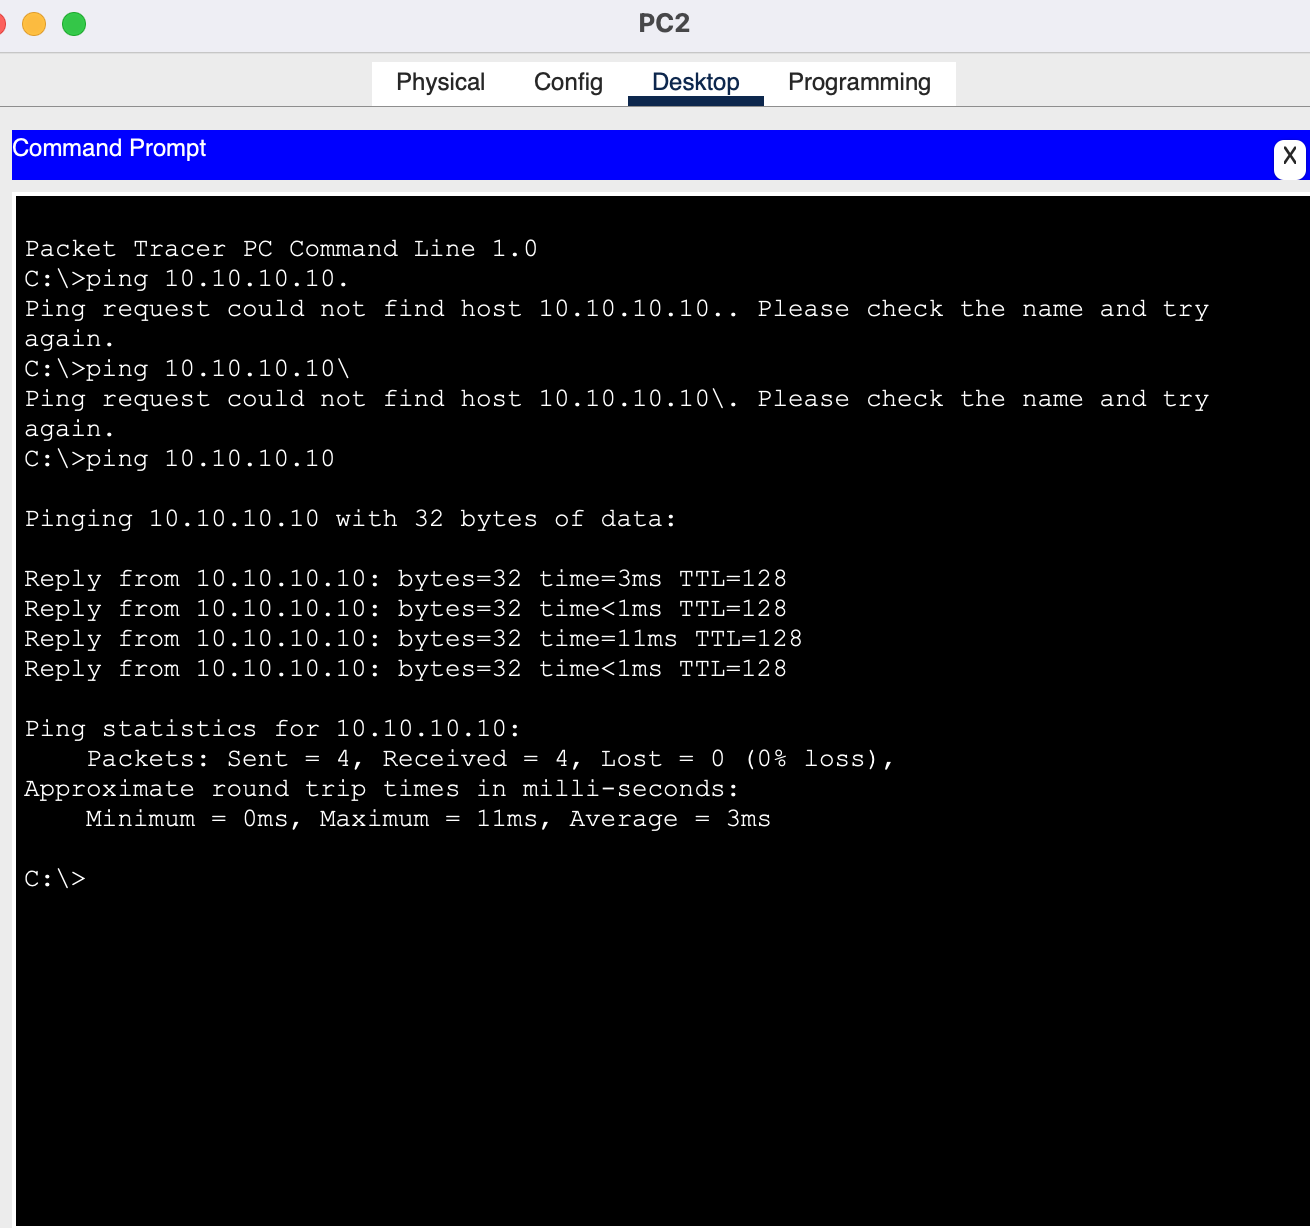
\includegraphics[scale=0.5]{pics/11.1.10_1.png}
                    \end{center}

                \item Ноутбук злоумышленника не имеет возможность отправлять ping запросы в локальной сети.
                    \begin{center}
                        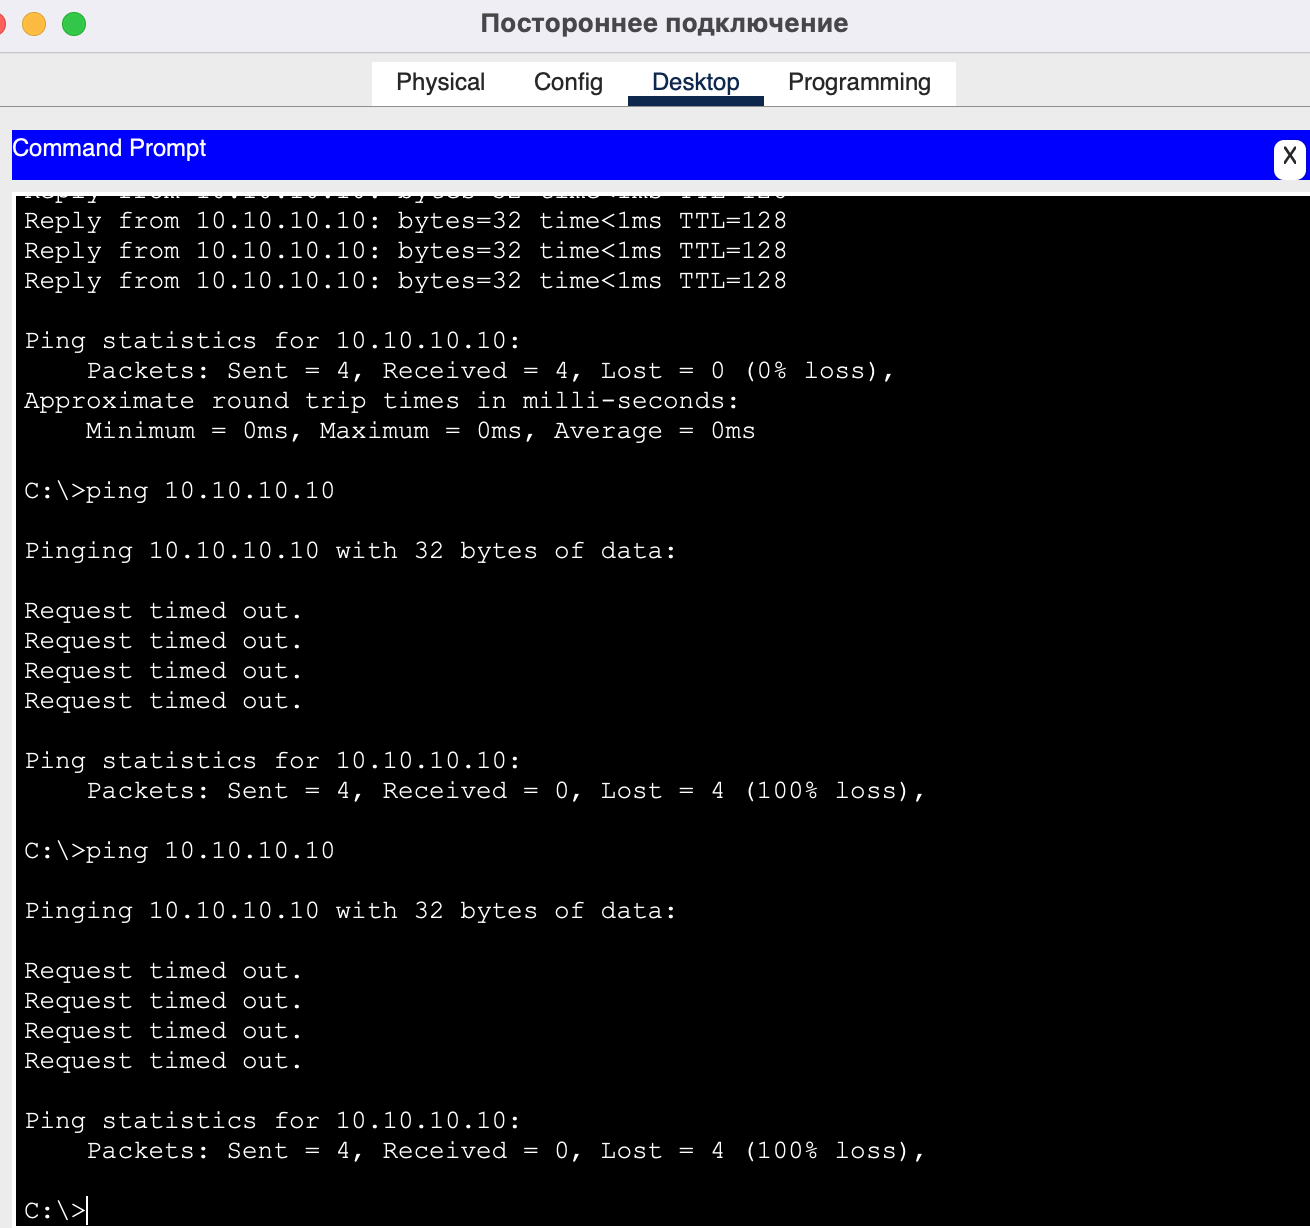
\includegraphics[scale=0.5]{pics/11.1.10_2.png}
                    \end{center}

                \newpage
                \item Вывод количества нарушений безопасности.
                    \begin{center}
                        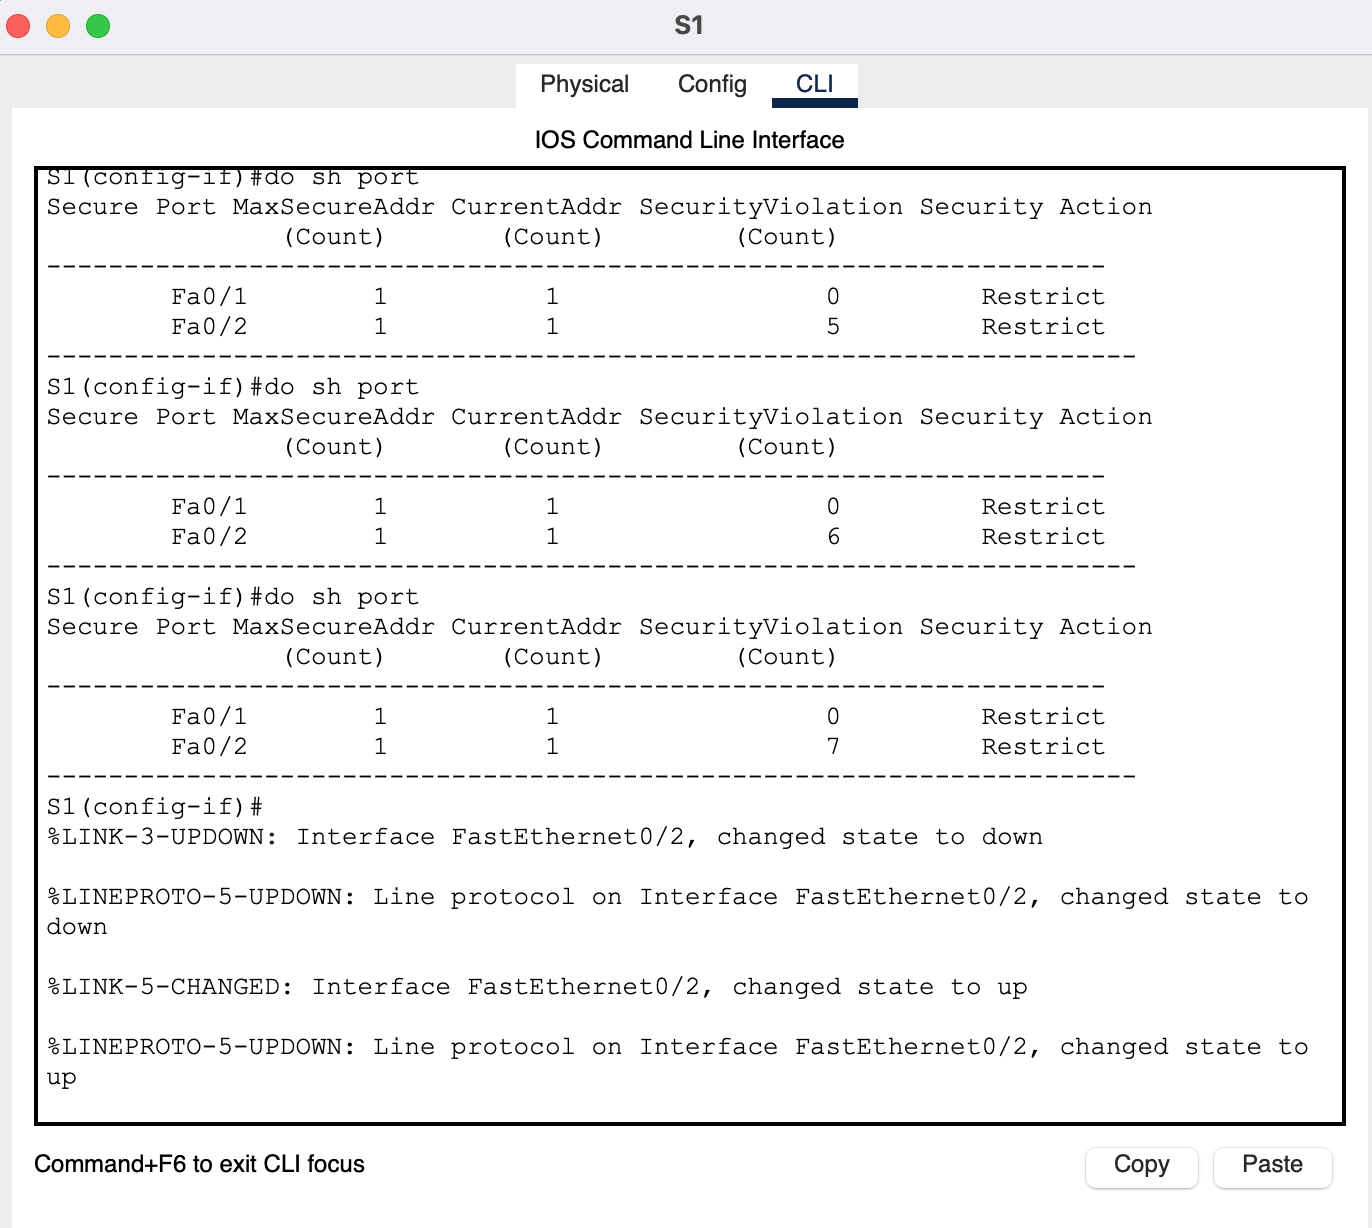
\includegraphics[scale=0.5]{pics/11.1.10_3.png}
                    \end{center}
            \end{itemize}
        \item \textbf{11.6.1 - Switch Security Configuration}
            \begin{itemize}
                \item \textbf{Список команд на sw-1}
                    \begin{lstlisting}
en
conf t
int range g0/1-2
switchport mode trunk
switchport nonegotiate
exit
vlan 100
name Native
exit
int range g0/1-2
switchport trunk native vlan 100
exit
int range f0/3-9, f0/11-23
shutdown
exit
vlan 999 
name BlackHole
int range f0/3-9, f0/11-23
switchport mode access
switchport access vlan 999
exit
int range f0/1-2, f0/10, f0/24
switchport port-security 
switchport port-security maximum 4
switchport port-security mac-address sticky
switchport port-security violation restrict
exit
int f0/1
switchport port-security mac-address 0010.11E8.3CBB
exit
int range g0/1-2
ip dhcp snooping trust 
int range f0/1-24
ip dhcp snooping limit rate 5
exit
int range f0/1-2, f0/10, f0/24
spanning-tree portfast
spanning-tree bdpuguard enable
                    \end{lstlisting}
                \item \textbf{Список команд на sw-2}
                    \begin{lstlisting}
en
conf t
int range g0/1-2
switchport mode trunk
switchport nonegotiate
exit
vlan 100
name Native
exit
int range g0/1-2
switchport trunk native vlan 100
exit
ip dhcp snooping vlan 10, 20, 99
int range f0/1-2, f0/10, f0/24
spanning-tree portfast
                    \end{lstlisting}
            \end{itemize}
    \end{enumerate}
\end{document}